
\section{Inbetriebnahme eines Osmocom Systems}
Für Inbetriebnahme des GSM Netzes waren einige Vorinstallationen sowie das Einrichten von Ubuntu 16.04.3 nötig. Im Folgenden wird das Vorgehen zur Einrichtung des Systems sowie die Inbetriebnahme des GSM Netzes beschrieben.

\subsection{Vorinstallationen}

\subsubsection{Ubuntu 16.04.3}
Zunächst wurde das Betriebssystem Ubuntu 16.04.3 auf einem Labor-Rechner installiert und eingerichtet.

\subsubsection{Git}
Da die Open-Source Projekte von OsmocomBB auf Git-Repositories liegen, wurde zunächst Git eingerichtet. Zur Versionskontrolle und Verwaltung des Codes wurde außerdem ein Team-eigenes Git Repository angelegt.

\begin{lstlisting}
sudo apt-get install git
\end{lstlisting}

\subsubsection{Softwarevoraussetzungen}
Osmocom empfiehlt zunächst die Einrichtung von einigen Bibliotheken und sonstigen, nötigen Abhängigkeiten als Voraussetzung für die Inbetriebnahme der GSM Komponenten. Diese wurden mittels Paketmanagers wie folgt installiert.

\begin{lstlisting}
sudo apt-get install libpcsclite-dev libtalloc-dev libortp-dev libsctp-dev 
libmnl-dev libdbi-dev libdbd-sqlite3 libsqlite3-dev sqlite3 libc-ares-dev 
libdbi0-dev libdbd-sqlite3 build-essentials libtool autoconf automake pkg-config 
libsqlite3-tcl sqlite-autoconf sqlite-autoconfg
\end{lstlisting}

Die die Fehler bezüglich Bumpversion nicht behoben werden konnten, wurden sie ignoriert. Dies zog keinerlei Konsequenzen hinsichtlich der Inbetriebnahme der GSM Komponenten nach sich.

Zusätzlich bedarf es der separaten Installation der Software Bibliotheken libosmo-abis, libosmocore und libosmo-netif. Diese wurden von den entsprechenden Git Repositories heruntergeladen und nach analogem Vorgehen installiert.

\begin{lstlisting}
git clone git://git.osmocom.org/<lib-source>
cd <lib-source>
autoreconf -fi
./configure
make
make install
sudo ldconfig
\end{lstlisting}

Trotz der sorgfältigen Installation einiger Softwarevoraussetzungen traten zusätzliche Abhängigkeiten bei der Installation einzelner GSM Komponenten auf, welche in \ref{GSM_Komp_Osmocom} beschrieben sind.

\subsubsection{Aktivierung der Verbindung zum USRP2}
Vor Installation des Treibers sollte zunächst die Netzwerkschnittstelle wie folgt aktiviert werden. Die default IP Adresse des Ettus USRP2 ist 192.168.10.2. 

\begin{lstlisting}
sudo ifconfig enp0s25 192.168.10.3
ping 192.168.10.2
\end{lstlisting}

\subsection{Installation einzelner GSM Komponenten}\label{GSM_Komp_Osmocom}
OsmocomBB hält detaillierte Beschreibungen zur Installation der GSM Komponenten bereit, welche zur Inbetriebnahme des in Rahmen dieser Arbeit verwendeten GSM Netzes herangezogen wurden. Im Folgenden wird die Installation und Einrichtung der GSM Komponenten genauer erläutert. 

\subsubsection{OsmoTRX}
Zur Kommunikation mit der Basisstation ist der osmoTRX Treiber nötig. Osmocom bietet diesen - meist wie die anderen Komponenten - im Git Repository an. Die Installation des Treibers erforderte die Bibliotheken \textit{$libusb-1.0-0-dev$, $uhd-host$, $libboost-dev$} und \textit{$libuhd-dev$}. Diese bieten die Suchfunktion \textit{uhd\_find\_devices}. Dadurch lässt sich testen, ob die Basisstation gefunden wird. Mittels \textit{osmo-trx} lässt sich der Treiber nach der Installation starten.

\begin{lstlisting}
git clone git://git.osmocom.org/osmo-trx
cd osmo-trx/
autoreconf -i
./configure
sudo make -j8
sudo make install
osmo-trx	
\end{lstlisting}

Zur Behebung der Warnung, die in Abbildung \ref{fig:UHDWarnung} zu sehen ist, wurde die Priorität in der Datei /etc/security/limits.conf gesetzt.

\begin{lstlisting}
@usrp   -  rtprio  50
\end{lstlisting}

\begin{figure}[h] %t=top b=bottom h=here p =eigene page
\centering
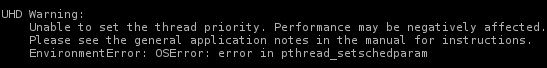
\includegraphics[width=15cm]{includes/uhd_usrp_warnung}
\caption{Fehlermeldung bezüglich der Thread Priorität in osmoTRX}
\label{fig:UHDWarnung}
\end{figure}

\subsubsection{OsmoBTS}
Die Installation von OsmoBTS erfolgte analog zur Einrichtung der anderen Osmocom Komponenten.

\begin{lstlisting}
git clone git://git.osmocom.org/osmo-bts.git
autoreconf -fi
cd osmo-bts
./configure
sudo make -j8
sudo make install
\end{lstlisting}

Zur Konfiguration wurden zunächst die Pfade der folgenden Variablen angepasst.

\begin{lstlisting}
PATH="/usr/local/sbin:/usr/local/bin:/usr/sbin:/usr/bin:/sbin:/bin:/usr/games:/usr/local/games"
PKG_CONFIG_PATH="/home/netpc06/libosmo-abis/"
LIBOSMOTRAU_CFLAGS="/home/netpc06/libosmo-abis/"
LIBOSMOTRAU_LIBS="/home/netpc06/libosmo-abis/"
\end{lstlisting}

\subsubsection{OpenBSC}
Weiterhin wurde OpenBSC installiert. Dazu wurde die Bibliothek libssl-dev (eigentlich unter libcrypto bekannt) vorausgesetzt.

\begin{lstlisting}
sudo apt-get install libssl-dev
git clone git://git.osmocom.org/openbsc
cd openbsc/
cd openbsc/openbsc/
autoreconf -i
./configure 
sudo make -j8
sudo make install
\end{lstlisting}

Zur Konfiguration von OpenBSC wurde eine Beispieldatei wie folgt angepasst (siehe Anhang \ref{Openbsc.cfg}). \textit{short name} und \textit{long name} beschreiben den Name des Netzwerks und wurden umbenannt. Die Option \textit{auth policy} wurde auf \textit{accept-all} gesetzt, um alle


\subsection{Starten des Systems}
